\subsection{The game description}

CrossWise is a simple 6X6 board game that has a maximum of four players in two teams, a vertical team and a horizontal team. Two teams always play against each other. On the side of the vertical team, all vertical lines on the game board are always noticed. And on the horizontal side, they always focus on the horizontal board lines. 

With regard to players' hands, every player has four tokens as a hand from the beginning. In each round, they have a chance to place a token on the chess board or to use a functional token to reach their purpose.

Furthermore, there are more following sections that describe the detail of the game rules, the game element involved, and the condition of winning a game.    

\subsubsection{Token}

This game is played with six different symbol tokens which have unique shapes and colors, and four different action tokens have their own functionality. This increases game variability and difficulties. The following description is about the utilization of symbol token and action token:

\begin{enumerate}
	\item\textbf{Symbol Token }\\
    The symbol tokens consist of six different shapes, for example, cross, pentagon, square, star, sun, and triangle. As you can see in the Figure \ref{fig:symbol tokens}. Each symbol token exists seven times in a round of a game. The main functionality of those symbol tokens is that player selects one of them as a placing token onto the chess board to occupy a position on the board. 
	
	\begin{figure}[h]
		\centering
		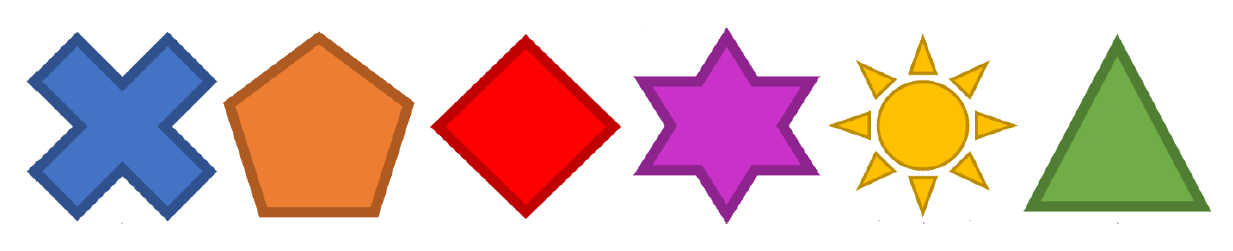
\includegraphics[width=0.8\textwidth]{image/Symbol tokens}
		\caption{All symbol tokens}
		\label{fig:symbol tokens}
	\end{figure}
	
	\item\textbf{Action Token }\\
	The action tokens consist of four different patterns, e.g., Remove, Shifter, Exchange, and Replace.
	Each of them exists three times in a round of a game. The description of those action tokens is shown below based on the order of the figure \ref{fig:action tokens}
	\begin{itemize}
		\item {Remove}\\
		The player moves a token of his choice on the board to another empty square of his choice (the square does not have to be adjacent).
		
		\item {Shifter}\\
		The player removes a token of his choice on the board. He takes the removed stone into his hand.
		
		\item {Exchange}\\
		The player swaps two tokens of his choice on the board with each other.
		
		\item {Replace}\\
		The player replaces a token of his choice on the board with one of his own tokens. He takes the replaced token into his hand.
		
	\end{itemize}
	
	\begin{figure}[h]
		\centering
		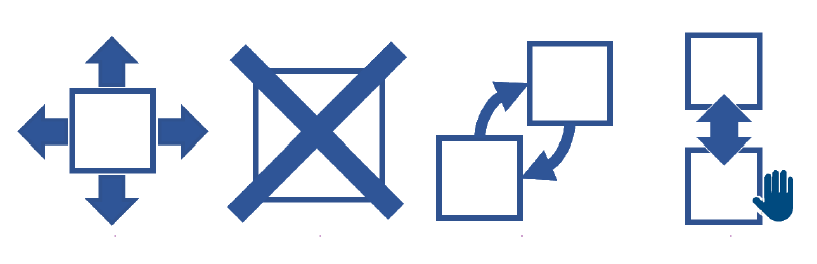
\includegraphics[width=0.6\textwidth]{image/Action tokens}
		\caption{Action tokens}
		\label{fig:action tokens}
	\end{figure}
	
\end{enumerate}

\subsubsection{Scoring Points}
In essence, scoring points has six combinations in this game. As you can see those combinations are under the table~\ref{tab:scoringPoints}. In each line, some combinations can appear simultaneously. Thus, the scoring points of a line depending on the combinations achieved in the respective line.

\begin{table}[h]
	\centering
	\begin{tabular}{|l|l|}
		\hline\xrowht[()]{10pt}
		Combinations          & Point    \\ 
		\hline\xrowht[()]{10pt}
		Six different symbols & 6 Points \\ 
		\hline\xrowht[()]{10pt}
		Two same symbols      & 1 Points \\
		\hline\xrowht[()]{10pt}
		Three same symbols    & 3 Points \\
		\hline\xrowht[()]{10pt}
		Four same symbols     & 5 Points \\ 
		\hline\xrowht[()]{10pt}
		Five same symbols     & 7 Points \\
		\hline
	\end{tabular}
	\renewcommand{\arraystretch}{4}
	\caption{A scoring points table.}
	\label{tab:scoringPoints}
\end{table}

\subsubsection{Player Mode}
This game has different player modes that can be only two players or four players to start a game. In addition, there are free combinations for each player that can be all human players, a mixture of human players and computer players, or all computer players. 

\subsubsection{The condition of winning a game}
There are two different approaches to reach winning a game. Generally speaking, the game should be ended when the game board is wholly occupied. However, if there is one team has completed six same tokens on a line on the chess board, then the game can be ended in advance and the winner appears. 

\begin{itemize}
	\item {Six same tokens}\\
    A team has arranged six same tokens on a board, then this team becomes the winner and the game is ended.
	
	\item {High Score}\\
    If there is no team that reaches six same tokens during the game, then scoring both teams at the end of the game. Which team has the higher score, the team is the winner. 
	
\end{itemize}